\documentclass{article}

\usepackage{graphicx}
\usepackage{tikz}
\usetikzlibrary{positioning}
\usetikzlibrary{decorations.markings}


\begin{document}
\title{Beispiel}
\author{Tim}
\maketitle
\newpage


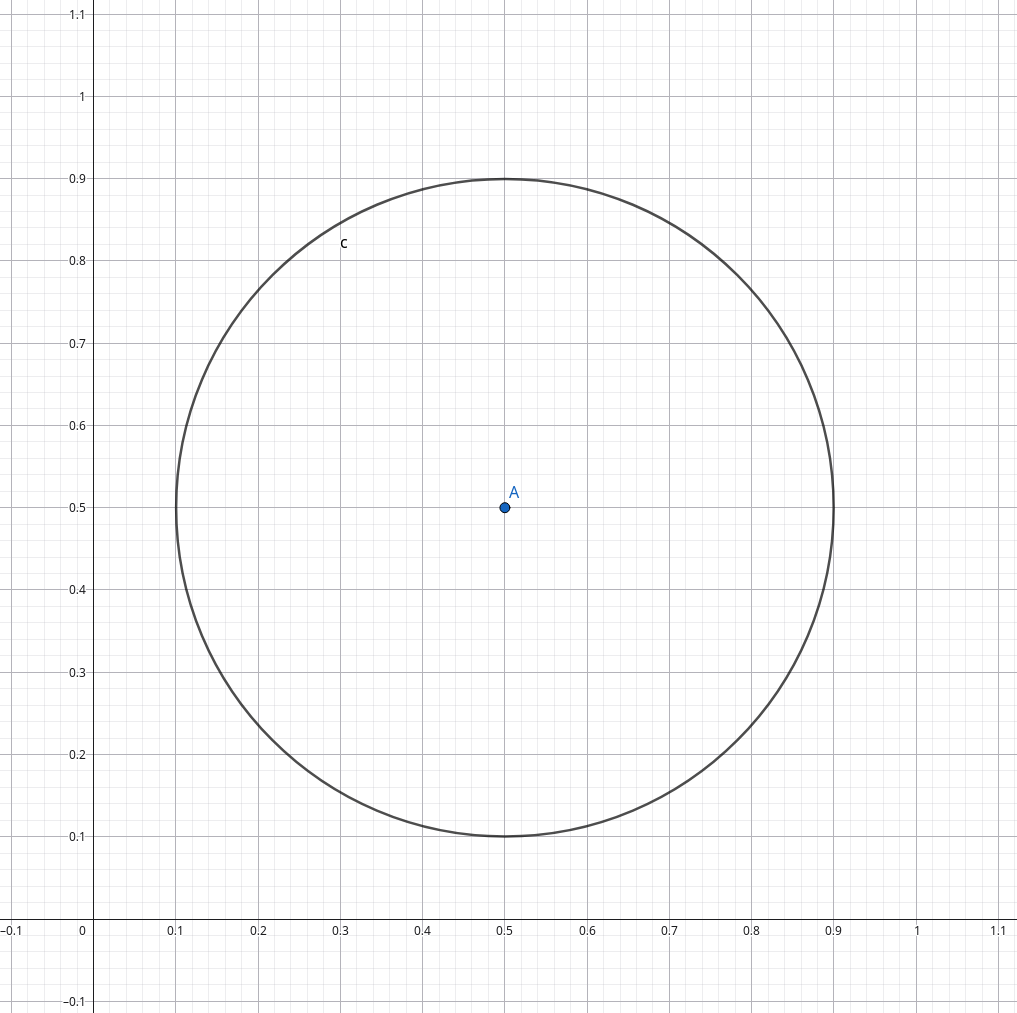
\includegraphics[scale=0.3]{Circle.png}

Frage: Liegt ein Punkt $P$ im Kreis?

Rechnerische Lösung:
\[ \sqrt{(x-0.5)^2 + (y-0.5)^2} < 0.4 \]



\newpage

\section{Lösung mit neuronalem Netz:}

\subsection{Netzstruktur}

\begin{tikzpicture} [thick, main/.style = {draw, circle}]

\node[main] (inputx) {x};
\node[main] (inputy) [below=2cm of inputx] {y};

\node[main] (hidden1) [right=2cm of inputx] {};
\node[main] (hidden2) [below=2cm of hidden1] {};
    
\end{tikzpicture}


\end{document}

